% Inspired by pgfmanual-en-tikz-arrows.tex bending/flexing examples.
\usetikzlibrary{arrows.meta,bending}

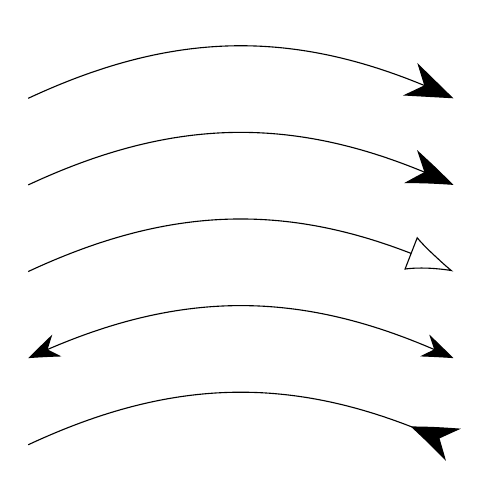
\begin{tikzpicture}[x=1cm,y=1cm]
  \draw[-{Stealth[length=6mm]}] (0,0) to[out=25,in=155] (5.4,0);
  \draw[-{Stealth[length=6mm,bend]}] (0,-1.1) to[out=25,in=155] (5.4,-1.1);
  \draw[-{Latex[open,length=6mm,bend]}] (0,-2.2) to[out=25,in=155] (5.4,-2.2);
  \draw[{Stealth[length=4mm,bend]}-{Stealth[length=4mm,bend]}] (0,-3.3) to[out=25,in=155] (5.4,-3.3);
  \draw[-{Stealth[length=6mm,bend,reversed]}] (0,-4.4) to[out=25,in=155] (5.4,-4.4);
\end{tikzpicture}
